\documentclass[11pt,a4paper]{article}
\usepackage[margin=2.4cm]{geometry}
\usepackage{amsmath,amssymb}
\usepackage{tikz}
\usetikzlibrary{arrows.meta,calc}
\usepackage{booktabs}
\usepackage[font=small]{caption}
\usepackage{parskip}
\newcommand{\Rey}{\mathit{Re}}
\newcommand{\om}{\omega}
\newcommand{\omh}{\hat\omega}

\title{Equilibria of Kolmogorov flow as an example for NKRoots.jl\\[2pt]\large The formulation, in a subspace where a state cannot drift}
\author{}
\date{12 November 2026}

\begin{document}
\maketitle

\section{The problem}

The flow is that of Golden (2026, section 2), two-dimensional and periodic on the square $[0, 2\pi)^2$, driven by the force $\sin(4y)\,\mathbf e_x$ at $\Rey = 40$. With the vorticity $\om = \partial_x v - \partial_y u$ his equation (2.3) is
\begin{equation}
\partial_t\om + \mathbf u\cdot\nabla\om = \frac{1}{\Rey}\nabla^2\om - 4\cos(4y).
\label{eq:vort}
\end{equation}
The velocity comes from the vorticity through the streamfunction, $\nabla^2\psi = -\om$, $u = \partial_y\psi$, $v = -\partial_x\psi$, with zero mean flow. An equilibrium is a root of
\begin{equation}
N(\om) = \mathbf u\cdot\nabla\om - \frac{1}{\Rey}\nabla^2\om + 4\cos(4y) = 0,
\label{eq:N}
\end{equation}
which is his (2.5) with the wave speed $c = 0$. One root is known in closed form, the laminar state $\om_L = -(\Rey/4)\cos(4y)$. Its velocity is along $x$ and its vorticity depends on $y$ alone, so the advection vanishes, and $-\nabla^2\om_L/\Rey = -4\cos(4y)$ cancels the forcing.

\emph{What the paper does, and what this example does.} The paper searches travelling waves and equilibria together. Its unknowns are the vorticity and the speed $c$, and a phase condition on the Newton step removes the motion along the shift. This example keeps to equilibria. The speed is not an unknown, and the shift is removed by a symmetry.

\section{The shift, and the subspace that removes it}

The forcing does not depend on $x$. If $\om(x, y)$ is an equilibrium, so is $\om(x + s, y)$ for every $s$. Differentiating $N(\om(x + s, y)) = 0$ in $s$ at $s = 0$ gives $N'(\om)\,\partial_x\om = 0$. The Jacobian at an equilibrium that depends on $x$ is singular, with $\partial_x\om$ in its null space, and Newton's method needs the shift fixed.

Let $R$ be the rotation of the square by half a turn about the origin, $(R\om)(x, y) = \om(-x, -y)$ (figure~\ref{fig:sym}, left). Each term of \eqref{eq:N} keeps it.
\begin{itemize}\setlength{\itemsep}{1pt}
\item \emph{The forcing.} $\cos(4y)$ is even in $y$ and does not depend on $x$, so $R\cos(4y) = \cos(4y)$.
\item \emph{The Laplacian.} Two changes of sign leave the second derivatives as they are, $\nabla^2 R\om = R\nabla^2\om$.
\item \emph{The advection.} If $\om$ is replaced by $R\om$, the streamfunction becomes $R\psi$, since the Laplacian commutes with $R$. A first derivative of a rotated field changes sign, so the velocity becomes $-R\mathbf u$ and the gradient $-R\nabla\om$. The two signs cancel in the product, $\mathbf u\cdot\nabla\om \to R(\mathbf u\cdot\nabla\om)$.
\end{itemize}
Hence $N(R\om) = R\,N(\om)$. The fields with $R\om = \om$ form a subspace $\mathcal S$, and $N$ maps $\mathcal S$ into itself. A search that starts in $\mathcal S$ stays there.

In $\mathcal S$ the shift is gone. The derivative $\partial_x\om$ of a field of $\mathcal S$ changes sign under $R$, so it is not in $\mathcal S$, and the Jacobian restricted to $\mathcal S$ does not have it in its null space. A shifted copy $\om(x + s, y)$ of a field of $\mathcal S$ that depends on $x$ is in $\mathcal S$ only for $s = \pi$, or for the shifts that the field is invariant to. Every root found in $\mathcal S$ solves \eqref{eq:N}, so it is an equilibrium. The price is that $\mathcal S$ holds only the equilibria with this symmetry, up to a shift. The others are out of reach of this example.

\begin{figure}[h]
\centering
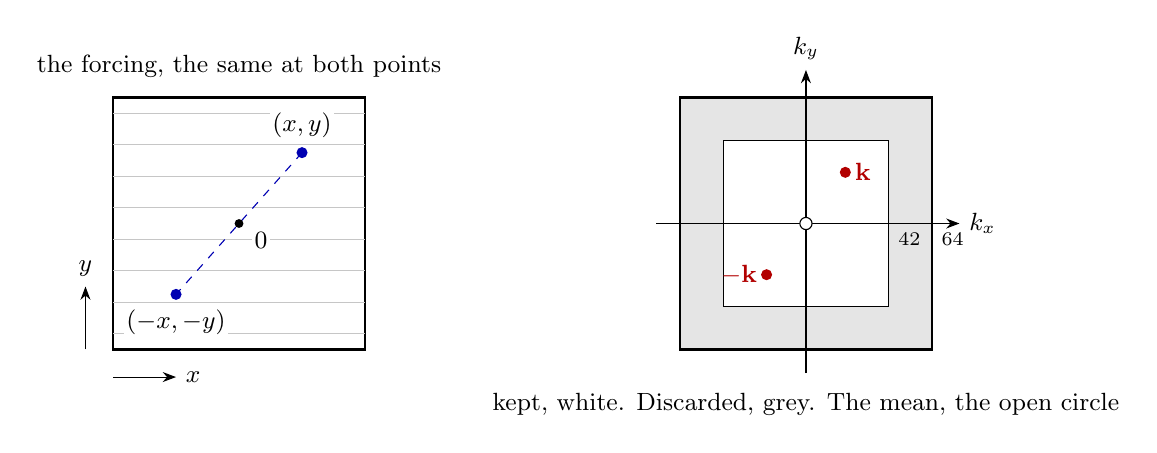
\begin{tikzpicture}[>=Stealth, scale=1.0]
  % ---- the square and the rotation ----
  \draw[thick] (-1.6,-1.6) rectangle (1.6,1.6);
  \foreach \y in {-1.4,-1.0,...,1.4} \draw[gray!45, thin] (-1.6,\y) -- (1.6,\y);
  \draw[dashed, blue!70!black] (0.8,0.9) -- (-0.8,-0.9);
  \fill (0,0) circle (1.6pt);
  \node[fill=white, inner sep=1pt] at (0.28,-0.22) {\small $0$};
  \fill[blue!70!black] (0.8,0.9) circle (2pt);
  \fill[blue!70!black] (-0.8,-0.9) circle (2pt);
  \node[fill=white, inner sep=1pt] at (0.8,1.25) {\small $(x, y)$};
  \node[fill=white, inner sep=1pt] at (-0.8,-1.25) {\small $(-x, -y)$};
  \draw[->] (-1.6,-1.95) -- (-0.8,-1.95) node[right] {\small $x$};
  \draw[->] (-1.95,-1.6) -- (-1.95,-0.8) node[above] {\small $y$};
  \node at (0,2.0) {\small the forcing, the same at both points};
  % ---- the Fourier plane ----
  \begin{scope}[shift={(7.2,0)}]
    \fill[gray!20] (-1.6,-1.6) rectangle (1.6,1.6);
    \fill[white] (-1.05,-1.05) rectangle (1.05,1.05);
    \draw[thick] (-1.6,-1.6) rectangle (1.6,1.6);
    \draw (-1.05,-1.05) rectangle (1.05,1.05);
    \draw[->] (-1.9,0) -- (1.95,0) node[right] {\small $k_x$};
    \draw[->] (0,-1.9) -- (0,1.95) node[above] {\small $k_y$};
    \fill[red!70!black] (0.5,0.65) circle (2pt) node[right] {\small $\mathbf k$};
    \fill[red!70!black] (-0.5,-0.65) circle (2pt) node[left] {\small $-\mathbf k$};
    \draw[fill=white] (0,0) circle (2.2pt);
    \node[below right] at (1.05,0) {\scriptsize $42$};
    \node[below right] at (1.6,0) {\scriptsize $64$};
    \node at (0,-2.3) {\small kept, white. Discarded, grey. The mean, the open circle};
  \end{scope}
\end{tikzpicture}
\caption{Left, the rotation $R$. Right, the Fourier modes of the $128\times128$ grid. In $\mathcal S$ the coefficients of $\mathbf k$ and $-\mathbf k$ are equal, and for a real field they are conjugate, so they are real.}
\label{fig:sym}
\end{figure}

\section{The discretisation}

The vorticity is stored on a grid of $128\times128$ points, $x_i = 2\pi i/128$, with the Fourier coefficients $\omh_{\mathbf k}$ of the fast Fourier transform, as in the paper. Derivatives and the velocity are computed in Fourier space, $\hat\psi_{\mathbf k} = \omh_{\mathbf k}/|\mathbf k|^2$, and the product $\mathbf u\cdot\nabla\om$ on the grid.

One projector $\Pi$ does three things to a field. It discards the modes with $|k_x| > 42$ or $|k_y| > 42$, the two-thirds rule. It removes the mean. It replaces each coefficient by its real part. The third is the projection on $\mathcal S$. The coefficient of $R\om$ at $\mathbf k$ is $\omh_{-\mathbf k}$, which for a real field is the conjugate of $\omh_{\mathbf k}$, so the symmetric part $(\om + R\om)/2$ has the coefficients $\mathrm{Re}\,\omh_{\mathbf k}$ (figure~\ref{fig:sym}, right). The rotation maps the grid to itself, $x_i \to x_{128 - i}$, so this holds on the grid exactly.

\emph{The two-thirds rule.} The product of two fields with wavenumbers up to 42 has wavenumbers up to 84. On a grid of 128 points a wavenumber $k$ above 64 appears as $k - 128$, and $84 - 128 = -44$ lies outside the kept band. The kept coefficients of the product are therefore exact.

\emph{The residual.} The unknown is the vorticity on the grid, 16\,384 numbers, and the residual is
\begin{equation}
G(\om) = \Pi\,N(\Pi\om) + (I - \Pi)\,\om .
\label{eq:G}
\end{equation}
On the range of $\Pi$ it is the equation \eqref{eq:N}, and on the rest it is the identity, as for the discarded modes and the mean in a usual pseudospectral code. A root of $G$ has $(I - \Pi)\om = 0$, so it is in $\mathcal S$, has no mean and no discarded mode, and solves the projected equation. The range of $\Pi$ has $(85^2 - 1)/2 = 3612$ real coefficients.

\emph{How the iterates stay in the subspace in floating point.} The Jacobian of \eqref{eq:G} is $\Pi N'(\Pi\om)\Pi + (I - \Pi)$. It has two blocks. On the range of $\Pi$ it is the Jacobian of the problem in $\mathcal S$, where the shift is gone. On the rest it is the identity. Rounding can put a small part of an iterate outside the range of $\Pi$. That part does not enter $N$, because $\Pi$ is applied first, and nothing of $N$ leaves the range, because $\Pi$ is applied last. The residual sees the stray part as $(I - \Pi)\om$, and the Newton step, through the identity block, subtracts it. So the stray part does not build up from one iteration to the next. With the Jacobian by finite differences it stays at the level of the rounding of the difference, and since it is part of the residual it is below the tolerance of the search at a root.

\section{The preconditioner}

The stiff part of $N$ is the viscous term. The preconditioner is the Stokes operator on the range of $\Pi$ and the identity elsewhere,
\begin{equation}
M = \Pi\Big(-\frac{1}{\Rey}\nabla^2\Big)\Pi + (I - \Pi), \qquad
\widehat{(M^{-1}f)}_{\mathbf k} = \frac{\Rey}{|\mathbf k|^2}\,\hat f_{\mathbf k}\ \ \text{on the range of }\Pi .
\end{equation}
It is diagonal in Fourier space, so $M^{-1}$ costs two transforms. The kept wavenumbers give the viscous term eigenvalues from $1/\Rey$ to $2\cdot42^2/\Rey = 88$, a spread of 3500. With the preconditioner the Jacobian becomes the identity plus the linearised advection times $M^{-1}$. The advection has one derivative and $M^{-1}$ removes two, so that product decays at large wavenumbers.

\emph{Right, not left.} The paper states that a preconditioner $\Rey\nabla^{-2}$ was critical to the success of GMRES, and applies it on the left of the Newton system, its equation (2.6). NKRoots preconditions on the right, so that the residual of GMRES is that of the Newton system itself and the trust region stays on the step in $\om$. The sign and the scale of $M$ do not matter, since the iterates do not change when $M$ is multiplied by a constant.

\section{The guesses}

As in the paper, a guess is random noise filtered in Fourier space. A field of independent normal numbers on the grid is transformed, the modes with $\max(|k_x|, |k_y|) > k_c$ are discarded with $k_c$ equal to 4, 5 or 6, the mean is removed, and the field is scaled to unit standard deviation. Here it is also made symmetric, by the real part of its coefficients, before the scaling. The seed of the random numbers and $k_c$ identify a guess.

\section{What the example shows}

\begin{enumerate}\setlength{\itemsep}{1pt}
\item \emph{The laminar state.} $G(\om_L)$ must vanish to rounding. This tests the signs, the transforms and the projector.
\item \emph{The energy balance.} Multiply \eqref{eq:N} by $\psi$ and average over the square. The advection gives $\langle\psi\,\mathbf u\cdot\nabla\om\rangle = 0$, the viscous term gives $\langle\om^2\rangle/\Rey$ after two integrations by parts, and the forcing gives $\langle 4\psi\cos(4y)\rangle = -\langle u\sin(4y)\rangle$. An equilibrium therefore has $D = I$, with the dissipation $D = \langle\om^2\rangle/\Rey$ and the input $I = \langle u\sin(4y)\rangle$. For the laminar state both are $\Rey/32$. The identity holds for the projected equation too, because $\psi$ is in the range of $\Pi$, so it checks every root to the tolerance of the search.
\item \emph{The globalisations.} Over a fixed list of guesses, how many searches converge with backtracking and with the hookstep under four rules, the classical rule of the radius, the greedy scan, the longest scan and the classical rule with the geodesic acceleration, at what cost and to what. The cost is counted in calls of $G$, residuals and Jacobian products together, since a product by finite differences is one call of $G$.
\item \emph{The preconditioner.} The iterations of GMRES on the same Newton systems with and without $M$, which tests the statement of the paper in this setting.
\item \emph{The fields.} The vorticity of one or two equilibria that are not the laminar state.
\end{enumerate}

\section{What I decided}

\begin{enumerate}\setlength{\itemsep}{1pt}
\item \emph{Equilibria only, in $\mathcal S$.} No wave speed and no phase condition. Equilibria without the symmetry are not found.
\item \emph{The square truncation} $|k_x|, |k_y| \le 42$ for the two-thirds rule, the largest band that the argument above allows on 128 points.
\item \emph{The norm.} The solver measures the residual and the step by the Euclidean norm of the values on the grid, which is 128 times the root mean square. The tolerance and the radius of the trust region are in that norm.
\item \emph{Double precision and one tolerance for GMRES.} The paper converges first in single precision with a tolerance that follows the residual. Here every search runs in double precision with the tolerance of GMRES fixed.
\item \emph{The Jacobian by finite differences} of $G$, the default of NKRoots, at one evaluation of $G$ per product.
\item \emph{The settings of the searches.} A Krylov space of at most 200 vectors, GMRES to a relative residual of $10^{-2}$, a tolerance of $10^{-8}$ on the residual in the norm of the grid, at most 80 iterations, and a first radius of 20 for the hookstep, against a guess of norm 128. Eight guesses, the seeds 1 to 8, each with backtracking and with the four rules of the hookstep.
\end{enumerate}

\subsection*{Reference}
M. Golden, \emph{A catalog of exact steady states in Kolmogorov flow}, arXiv:2609.27062 (2026).

\end{document}
